%\glossary{name=Standard Model, description=Standard Model}
\vspace{0.015\textheight}
In this chapter, the benchmark theory of elementary particle physics, the Standard Model (SM), is further described with the focus on different interactions. Then, some limitations of the SM are described. A prominent theory model, Supersymmetry (SUSY), which attempts to supersede the SM, is introduced as a motivation for this study. Next, the philosophy of signature-based searches and their advantages are described, and this leads to a motivation for the study of the photon + jets signature. Finally, photon + jets production under the SM and SUSY is explained.

\section{Fundamental Interactions}
\vspace{0.03\textheight}
\subsection{Electromagnetic Interaction}
It should be evident now that the electromagnetic (EM) interaction occurs via the exchange of photons. Particles with charge, positive or negative, may interact with other charged particles by exchanging photons. Particles with the same charge tend to repel each other, whereas particles with opposite charge tend to attract. The photon is massless and travels at the speed of light. Quantum Electrodynamics (QED), an abelian gauge theory with the symmetry group U(1), successfully describes all phenomena involving charged particle interactions via the exchange of photons. The electromagnetic \newterm{coupling}, or the strength of the interaction, is given by $\alpha_{em} = \frac{e^{2}}{4\pi\epsilon_{0}\hbar c} = \frac{1}{137}$, where $e$ is the electric charge of the electron, $\epsilon_{0}$ is the permitivity of free space, $\hbar$ is the reduced Planck constant, and $c$ is the speed of light. Figure~\ref{fig:LeptonInteraction} shows the interaction of an electron with a photon, where the photon is absorbed or emitted and the electron's momentum is changed. QED is one of the few complete and most accurate theories to date.

\begin{figure}[htb!]
 \centering
 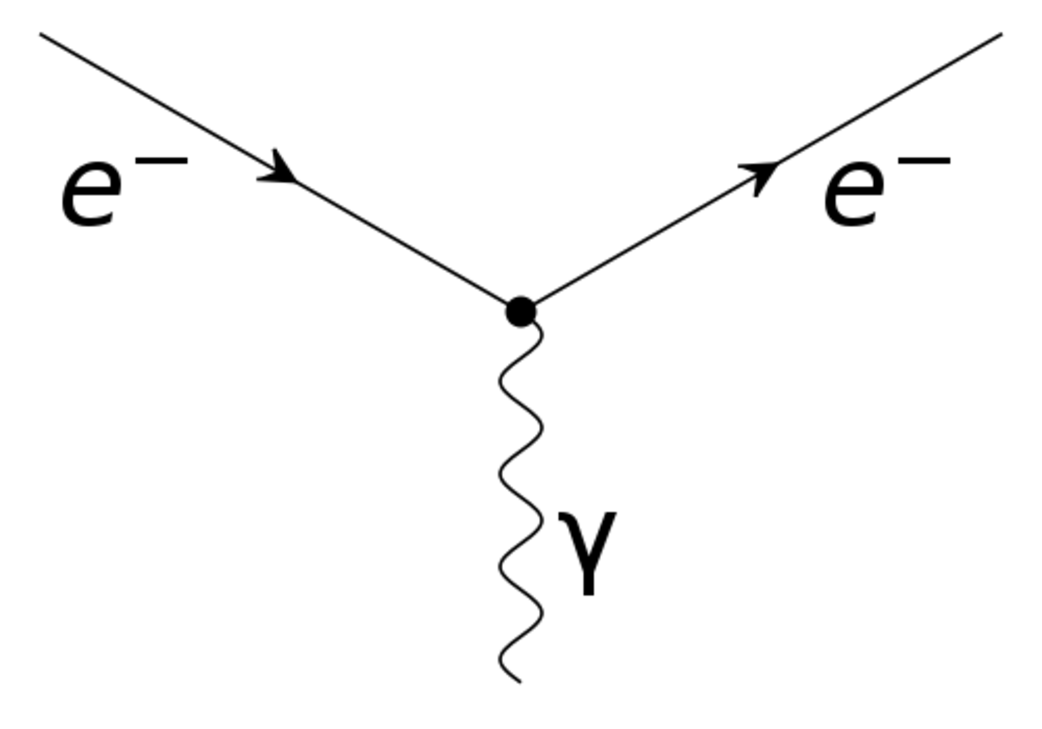
\includegraphics[scale=.25,keepaspectratio=true]{./LeptonInteraction.pdf}
 % LeptonInteraction.png: 500x350 pixel, 72dpi, 17.64x12.35 cm, bb=0 0 500 350
 \caption{Electron-photon interaction.}
 \label{fig:LeptonInteraction}
\end{figure}

\subsection{Strong Interaction}\label{sec:StrongInteraction}
As mentioned in the previous chapter, a fundamental question of the early explorers of the nucleus was how nuclei can stay stable with so many positively charged protons packed within a distance of a few femtometers (1 fm = $10^{-15}$ m). The answer was a force much stronger than the electromagnetic interaction, but with a very short range confined to the nuclear scale. This force is called the \newterm{strong} force. The strong force carriers, gluons, mediate the interactions between the quarks. The color charge of quarks, in addition to their electric charge, allow them to participate in strong interactions. Both gluons and quarks carry the color charge. Gluons are the quanta of the color field that bind quarks in nucleons and also nucleons into nuclei. Strong interactions preserve the color charge and are mathematically explained by the non-abelian SU(3) gauge symmetry under Quantum Chromodynamics (QCD). At the strong interaction scale of $\Lambda \sim$~200~MeV, the hadrons are composed of quarks and gluons. The \newterm{strong coupling}, which defines the strength of the strong interaction, is energy scale dependent, i.e. at higher energies the coupling decreases as in Eq.~\ref{eqa:QCDasymptoticFreedom}. This is termed \newterm{asymptotic freedom} (see Fig.~\ref{fig:RunStrongCoupling}).

\begin{figure}[p]
 \centering
 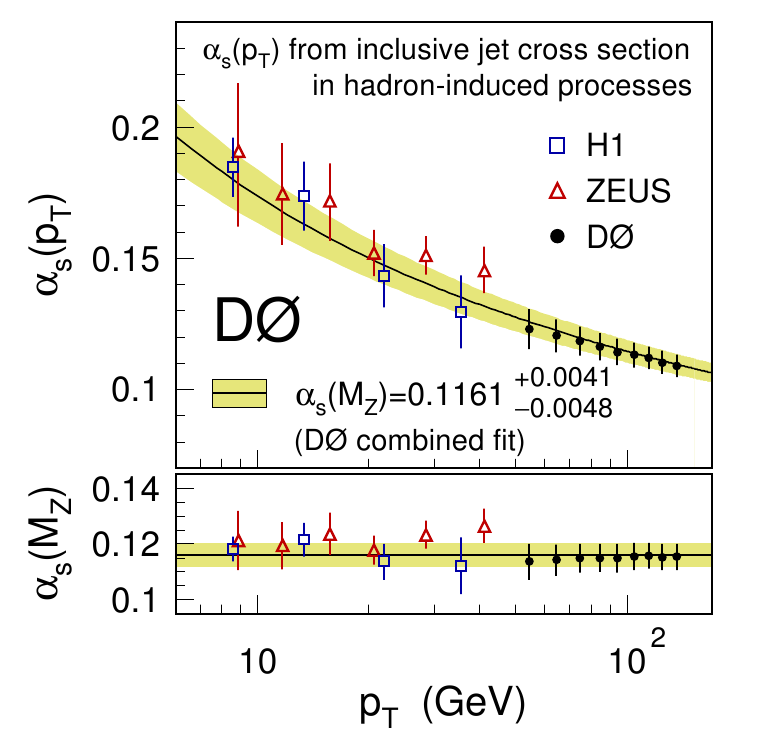
\includegraphics[scale=0.75]{./RunningStrongCoupling.png}
 % RunningStrongCoupling.png: 770x739 pixel, 96dpi, 20.37x19.55 cm, bb=0 0 577 554
 \caption{A recent D\O~measurement of the strong coupling constant, $\alpha_{s}$, as a function of \pt (top) and at the mass of the $Z$ boson, $M_Z$ (bottom). Measurements from the HERA experiment are overlaid for comparison. The error bars indicate combined statistical + systematic uncertainties~\cite{pap:D0_StrongCoupling}.}
 \label{fig:RunStrongCoupling}
\end{figure}

Asymptotic freedom allows the study of QCD processes using perturbation theory at high energies (see Section~\ref{sec:pQCD}). The coupling parameter of QCD interactions (\alphas) is a \newterm{running} constant (energy dependent) and to lowest order is described by Eq.~\ref{eqa:QCDasymptoticFreedom}. Here, $N_{f}$ is the number of quark flavors, $\Lambda$ is the QCD scale parameter, and $Q^{2}$ is the momentum transfer (energy) scale.

\begin{equation}
 \alpha_{s} (Q^{2}) =\frac{12\pi}{(33 - 2 N_{f})\log(Q^{2}/\Lambda^{2})}
 \label{eqa:QCDasymptoticFreedom}
\end{equation}

Quarks are not observed individually, but are always bound with other quarks or antiquarks in composite particles. If one attempts to separate quarks that are close to each other, they form color-neutral particles: mesons or baryons. This property of quarks and antiquarks to combine to form color-neutral particles is known as \newterm{color confinement}.

\begin{figure}[htb!]
 \centering
\subfigure[]{
 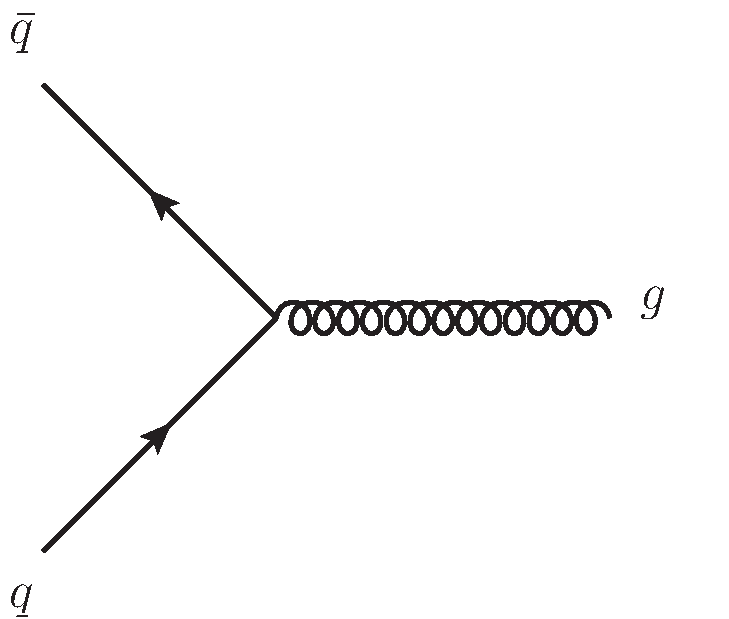
\includegraphics[scale=0.3,keepaspectratio=true]{images/QCD_vertices_1.pdf}
}
\subfigure[]{
 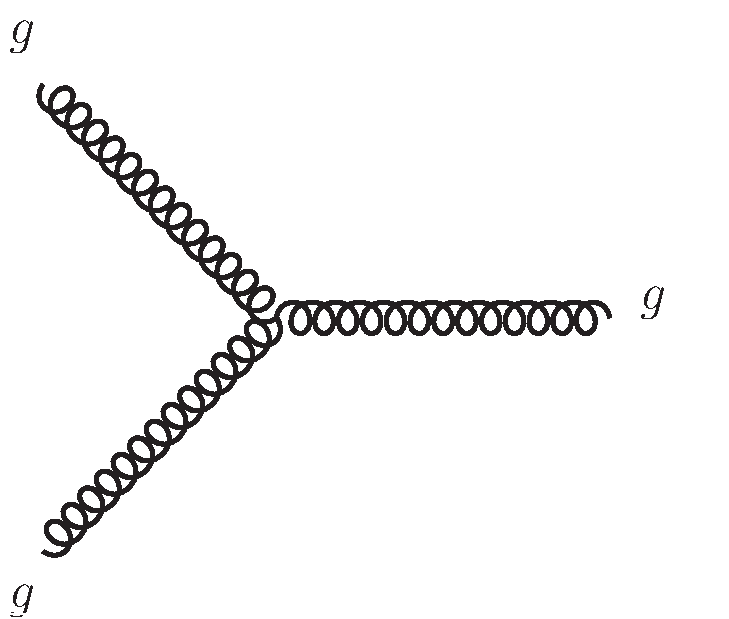
\includegraphics[scale=0.3,keepaspectratio=true]{images/QCD_vertices_2.pdf}
}
\subfigure[]{
 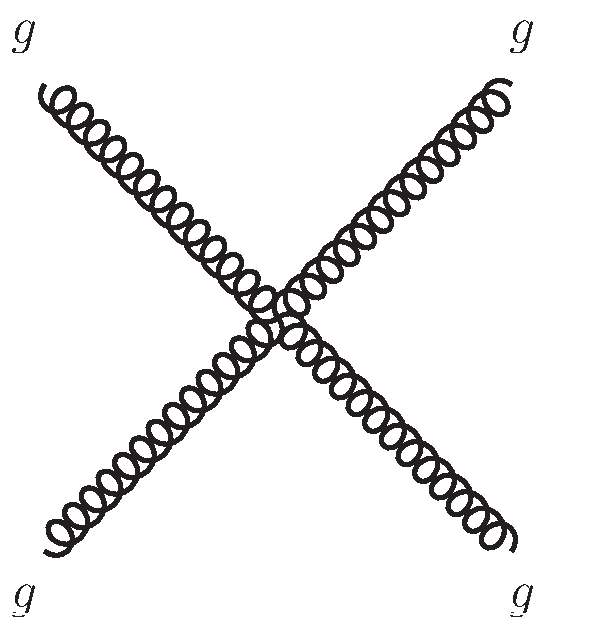
\includegraphics[scale=0.3,keepaspectratio=true]{images/QCD_vertices_3.pdf}
}
\caption{Quark and gluon interaction vertices under QCD.}
\label{fig:FeynQCDGluonCoupling}
\end{figure}

As shown in Fig.~\ref{fig:FeynQCDGluonCoupling}, the gluons (\particle{g}) can couple only to quarks or other gluons. The QCD Lagrangian is defined by
\begin{equation}
 {\cal L}_{QCD} = -\frac{1}{4} F_{a}^{\mu\nu} F_{a\mu\nu}+\bar{\Psi_{j}}(i\gamma_{\mu}D^{\mu}_{jk}-M_{j}\delta_{jk})\Psi_{k}
%X_i^{\phantom{i}j}\\\%this is a much better tech to get the superscript and subscript gets the same size
%X^j_{\phantom{j}i}\\
\end{equation}
where $D^{\mu}_{jk}$ is the covariant derivative given by
\begin{equation}
 D^{\mu}_{jk} = \delta_{jk}\partial^{\mu}+ig(T_{a})_{jk}G_{a}^{\mu}
\end{equation}
and $F_{a}^{\mu\nu}$ is the gluon field tensor, $\Psi_{k}$ represents the quark fields, $M$ represents the quark mass matrices, $g$ is the strong coupling constant, $G_{a}^{\mu}$ represents the gluon fields, and the $T$ are SU(3) generators. They follow the commutation relationship
\begin{equation}
 [T_{i},T_{j}]=if_{ijk}T_{k}.
\end{equation}
Here, the $f_{ijk}$ are the QCD structure constants. The \newterm{gamma matrices} ($\gamma$) are defined in the Dirac representation as:

\begin{equation*}
 \gamma^{0}=\left(
\begin{array}{ccc}
I & 0\\
0 & -I
\end{array}
\right),\quad
\gamma^{i}=\left(
\begin{array}{ccc}
0 & \sigma_{i}\\
-\sigma_{i} & 0
\end{array}
\right),\quad
\gamma^{5}=\left(
\begin{array}{ccc}
0 & I\\
I & 0
\end{array}
\right),
\end{equation*}
where $I$ is the $2\times2$ identity matrix and $\sigma_{i}$ are the Pauli matrices,
\begin{equation*}
 \sigma_{1}=\left(
\begin{array}{ccc}
0 & 1\\
1 & 0
\end{array}
\right),\quad
\sigma_{2}=\left(
\begin{array}{ccc}
0 & -i\\
i & 0
\end{array}
\right),\quad
\sigma_{3}=\left(
\begin{array}{ccc}
1 & 0\\
0 & -1
\end{array}
\right).
\end{equation*}

\subsection{Electroweak Interaction}
The electromagnetic and strong forces were enough to understand and explain many aspects of nature. However, the proposal of the \newterm{weak force} by Enrico Fermi solved the mystery of \newterm{beta decay},\footnote{Spontaneous emission of an electron or a positron by a nucleon in the atomic nucleus} which baffled scientists for a long time. The weak force allows a quark to change its flavor by exchanging a virtual boson (a $W$ or a \Z boson). The weak interactions of the first generation of leptons are shown in Fig.~\ref{fig:WeakInteractionVertices}. One of the major achievements of the SM is that the electromagnetic and the weak interaction are described by a single theory, the electroweak theory. The discovery of the \W and \Z intermediate vector bosons at CERN gave tremendous support to the theory. The \newterm{electroweak interaction} is implemented by a gauge theory based on the SU(2)$_\mathrm{L}$~$\times$ U(1)$_\mathrm{Y}$ group (where the \textit{L} indicates that the weak force couples only to the \newterm{left-handed} particles). A particle is \newterm{right-handed} if the direction of its spin is the same as the direction of its motion (see Fig.~\ref{fig:Helicity}). It is left-handed if the directions of spin and motion are opposite. %This group symmetry is spontaneously broken via the Higgs mechanism.

\begin{figure}[h]
 \centering
\subfigure[]{
 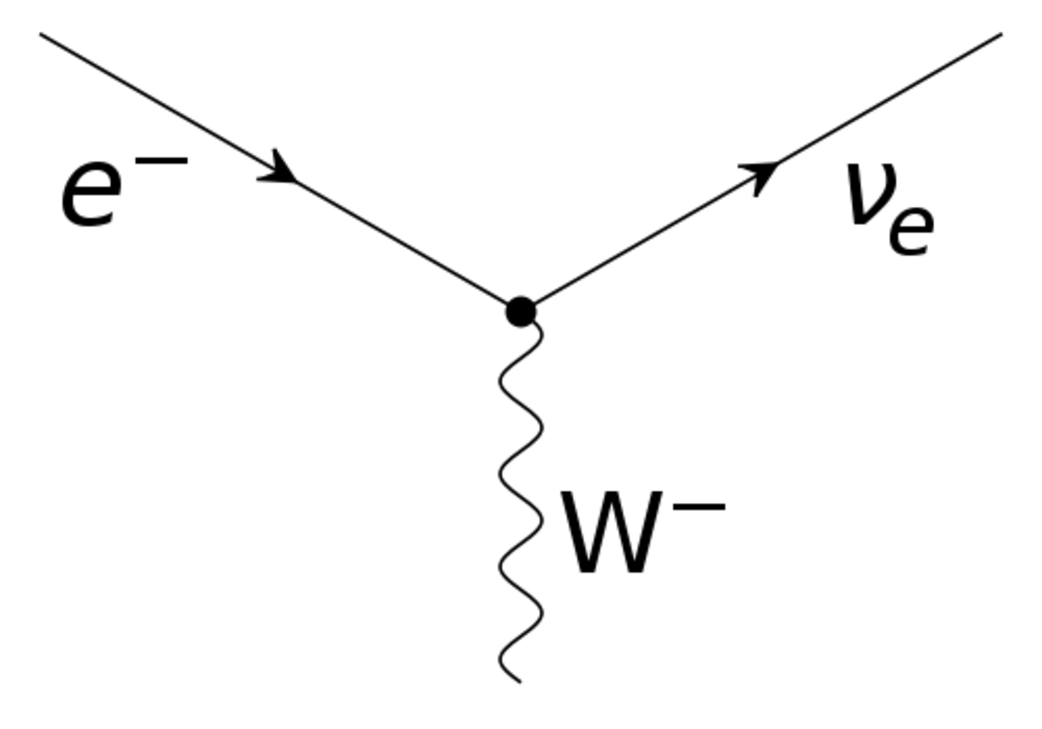
\includegraphics[scale=0.25,keepaspectratio=true]{./WeakInteractionVertex1.pdf}
}
\subfigure[]{
 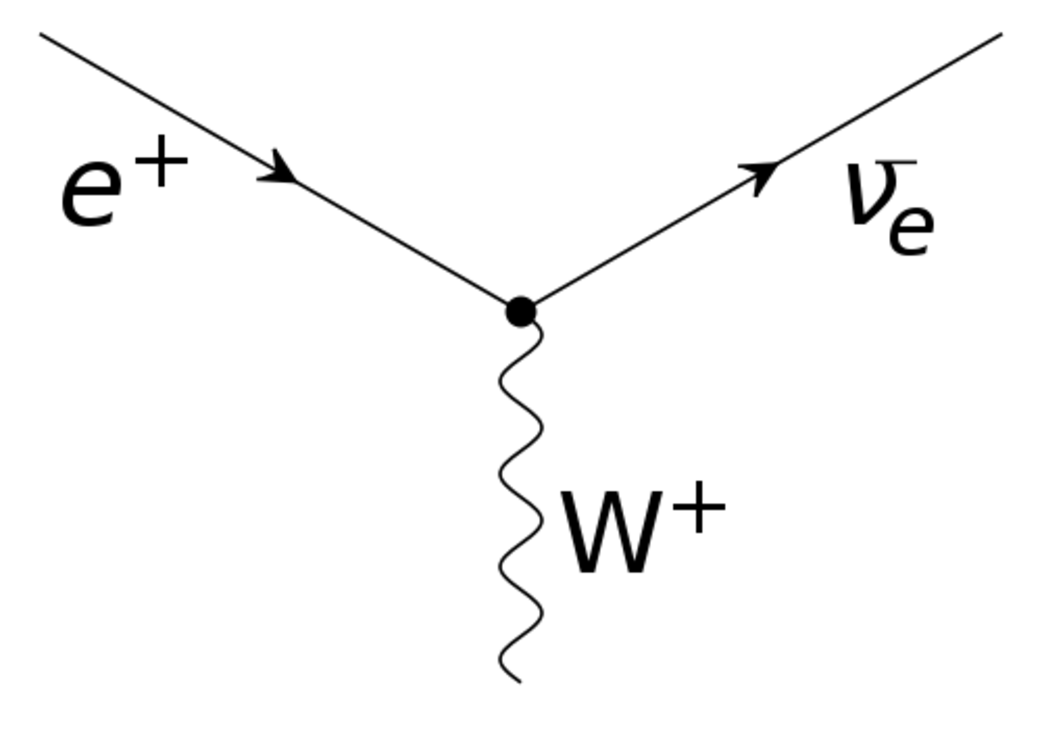
\includegraphics[scale=0.25,keepaspectratio=true]{./WeakInteractionVertex2.pdf}
}
\subfigure[]{
 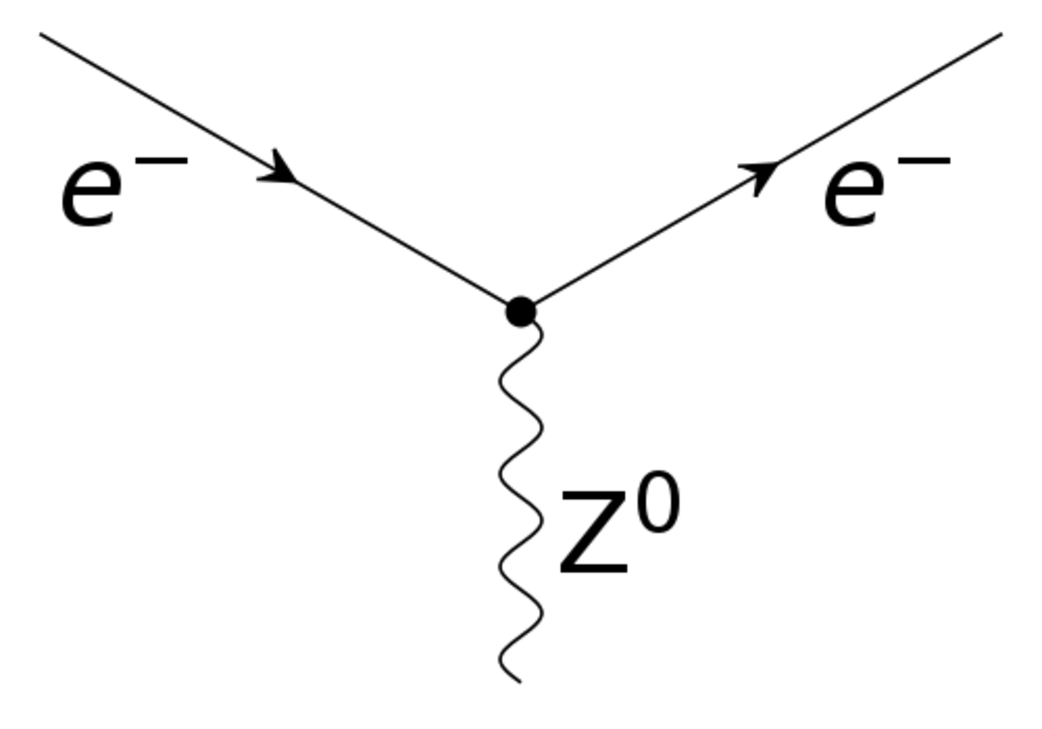
\includegraphics[scale=0.25,keepaspectratio=true]{./WeakInteractionVertex3.pdf}
}
 \caption{Weak interaction vertices of the first generation leptons.}
 \label{fig:WeakInteractionVertices}
\end{figure}

\begin{figure}[h!]
\vspace{3ex}
 \centering
 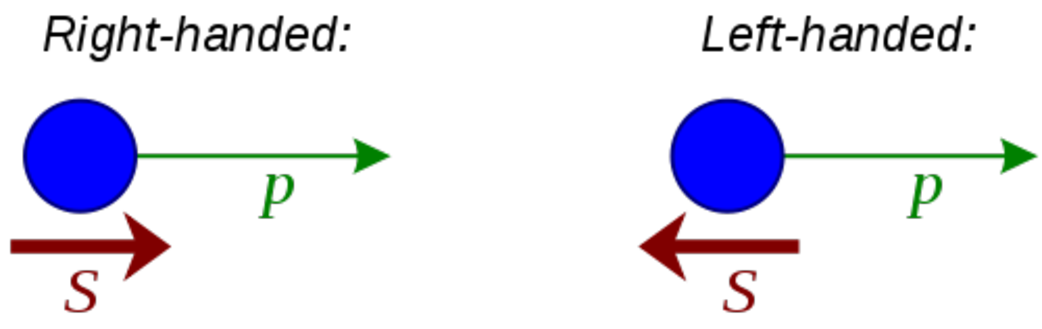
\includegraphics[scale=0.8,keepaspectratio=true]{./Helicity.pdf}
 % Helicity.png: 500x158 pixel, 72dpi, 17.64x5.57 cm, bb=0 0 500 158
 \caption{A particle is left-handed or right-handed based on the alignment of its spin ($S$) and momentum ($p$).}
 \label{fig:Helicity}
\end{figure}

The \newterm{weak interaction} is due to the exchange of the heavy \W and \Z bosons. For example, beta decay is possible only via the weak interaction. In reality, a down quark in a neutron ($udd$) decays into an up quark, converting it to a proton ($uud$) via an exchange of $W^{-}$ boson. The $W^{-}$ boson subsequently decays into a electron ($e^{-}$) and an electron antineutrino ($\bar\nu_{e}$). The weak interaction allows a quark to change its flavor by emission or absorption of a vector boson (\W). A lepton or a quark can readily absorb or emit a \Z boson without changing its flavor.

\subsection{Gravity}
Gravity is described here only for the completeness of the discussion. Gravity is by far the weakest of all the forces (see Table~\ref{tab:summary_of_four_forces}). As a result, it has no measurable effect on a subatomic scale. So far, the SM has not been able to extend its Lagrangian to incorporate gravity. In addition, the force-mediating particle of gravity, the graviton, has yet to be discovered.

\subsection{Unification of Forces}
Similar to the unification of the electromagnetic and weak interactions into the electroweak theory, \newterm{Grand Unification Theories} (GUTs)~\cite{pap:GUTtheory} predict that the SM fundamental interactions (electromagnetic, weak, and strong) unite at an extremely high energy scale (see Fig.~\ref{fig:TOE_ForceUnified}). Unifying gravity with the other three interactions forms a \newterm{Theory of Everything} (TOE) \cite{pap:TOE}.

\begin{figure}[p]
 \centering
 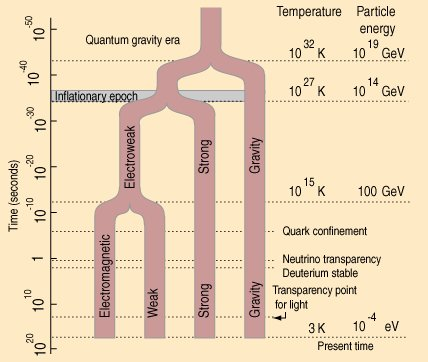
\includegraphics[scale=0.99 ,keepaspectratio=true]{./guts_forceUnification2.jpg}
 % guts_forceUnification.png: 540x476 pixel, 72dpi, 19.05x16.79 cm, bb=0 0 540 476
 \caption[Unification of the fundamental forces at extremely high energies.]{A theoretical prediction of the unification of the fundamental forces at extremely high energies. The energy limit of current particle accelerators is about 10$^{12}$~eV, making it impossible to test such theories.}
 \label{fig:TOE_ForceUnified}
\end{figure}

\subsection{Higgs Mechanism}\label{sec:EWKSymmetryBreaking}
The SM proposes that the mass of the observed particles arises from the interaction (coupling) of particles with the \newterm{Higgs field}, which has a non-zero \newterm{vacuum expectation value} (VEV). A naive picture is that the Higgs field exerts some amount of resistance as the particles traverse the field, and hence the field gives rise to the inertial mass that is observed. The resistance is different for different particles. Of course, other kinds of interactions like the strong interaction can contribute to the resulting measured mass.

The Higgs mechanism was incorporated into the SM to generate masses for the heavy vector bosons and eventually the lighter fermions. This was achieved by breaking the electroweak symmetry via Higgs mechanism. As a result a new scalar particle (spin-0) called the Higgs boson is predicted.

The Higgs boson (\particle{H}) is the only particle predicted by the SM that has yet to be observed experimentally. Like all other particles, the Higgs boson acquires its mass by interacting with the Higgs field. Direct searches at the Tevatron and LEP (Large Electron-Positron Collider at CERN) have shown the mass of the \particle{H} to be greater than 114~\massunits. Recent Tevatron data have excluded a Higgs mass between 158~$<M_{H}<175$~\massunits at the 95\% confidence level \cite{pap:HiggsLimits}.

\section{Limitations of the \SMtext}
The SM has been tested extensively by experimental data. So far, no evidence contradicting SM predictions has been observed. Yet, there are many questions that are not addressed or verified by the SM. If one compares the strength of the four fundamental forces (see Table~\ref{tab:summary_of_four_forces}), it is evident there are two widely separated scales. The gravitational force is proportional to the inverse of the distance squared, yet its interaction is associated with a huge mass scale called the \newterm{Planck scale} ($\sim$10$^{19}$~GeV), which makes the interactions very weak. On the other hand, the \newterm{electroweak scale} (\mbox{$\sim$246 GeV}) sets the masses for $W$ and $Z$ bosons to be $\sim$80~\massunits and $\sim$91~\massunits, respectively. This, in its simplest manifestation, is known as the \newterm{hierarchy problem}.

\begin{figure}[htb!]
 \centering
\subfigure[]{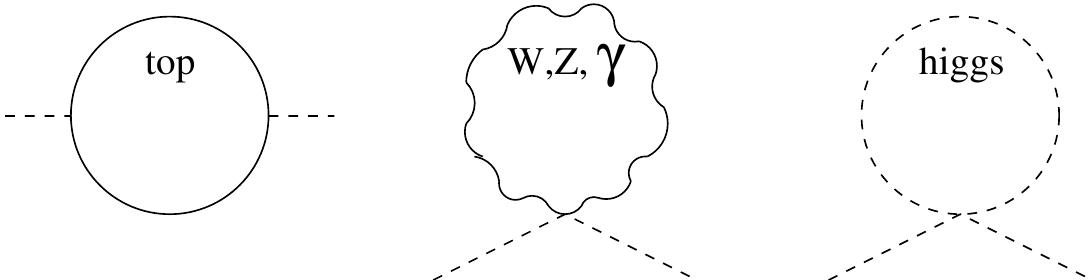
\includegraphics[keepaspectratio=true,scale=0.5]{./SMHiggsDivergentContributions.png}}\\[1ex]
\subfigure[]{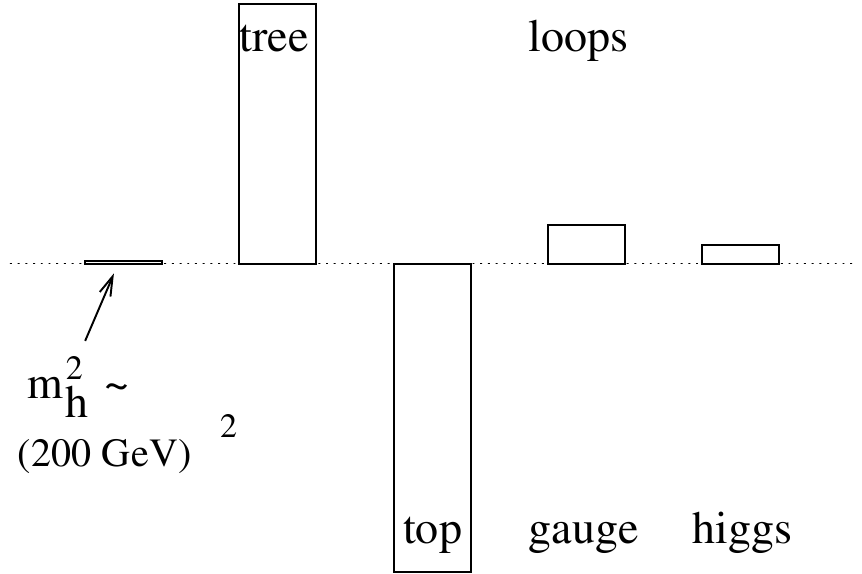
\includegraphics[keepaspectratio=true,scale=0.4]{./CorrectionsToHiggsMass2.png}}
\caption{(a) The most significant quadratically divergent contributions to the Higgs mass in the Standard Model and (b) the fine tuning required to obtain an acceptable Higgs mass in the Standard Model with cut-off 10~TeV.}
\label{fig:SMHiggsDivergentContributions}
\end{figure}

Another manifestation of the hierarchy problem is the undesirable large loop corrections to the Higgs mass as shown in Fig.~\ref{fig:SMHiggsDivergentContributions}. Furthermore, although there is plenty of evidence for electroweak symmetry breaking, the exact mechanism is not confirmed and the Higgs boson's existence has not been verified. In addition to these, there are other questions that need to be answered. Below are some of those questions.
\vspace{-0.01\textheight}
\begin{singlespace}
\begin{enumerate}
 \item It provides no prediction of the masses of the fundamental particles: the quarks and leptons.
 \item It does not explain the existence of two extra families of leptons and quarks, nor why there are only three families.
 \item It does not explain why gravity is so weak, and it is not able to describe its effects at the quantum level.
 \item The neutrinos were assumed to be massless. Yet recent experimental results show evidence of neutrino oscillations, which indicate that neutrinos may have a tiny but non-zero mass.
 \item There is no natural candidate for \newterm{dark matter}. Cosmology and astronomy suggests that 70\% of the universe is \newterm{dark energy} and another 25\% is made of \newterm{dark matter}, meaning only 5\% of visible matter is explained by the SM.
\end{enumerate}
\end{singlespace}

There are numerous new theory models attempting to address these shortcomings, like \newterm{Supersymmetry} (SUSY) and \newterm{Technicolor} \cite{pap:TechnicolorModel}. Since the production of a photon in association with jets is so fundamental, it is present in almost all such theory models. Among those theory models, SUSY has become a leading candidate and is being extensively studied by physicists.

\section{Supersymmetry (SUSY)}\index{SUSY}
Supersymmetry is one of the promising theory models attempting to supersede the SM. It is described in detail in the literature \cite{pap:SUSY_SMartin, pap:SUSY_IJRAitchison}. It assumes there is another physical symmetry beyond those included in the SM. By the introduction of heavier partners for all SM particles, SUSY is able to cancel the unphysical large loop corrections to the Higgs mass. It also provides an answer for why the weak force is far stronger than gravity (the hierarchy problem) (see Table~\ref{tab:summary_of_four_forces}). Furthermore, by unifying three of the SM gauge interactions (the weak interaction, strong interaction, and electromagnetic interaction) and having natural candidates for the dark matter, it is appealing to study.

\subsection{SUSY Particles}
The theory proposes the existence of supersymmetric particles (superpartners) for all the \SM particles. For each type of \SM boson, there is a fermionic superpartner and vice versa as shown in Fig.~\ref{fig:SM_SUSY_Particles}. The bosonic counterparts to the SM fermions get an ``s'' prefix (lepton~$\to$``slepton'', ``quark''~$\to$ ``squark'') and the fermionic counterparts to SM gauge bosons get an ``ino'' suffix (``gauge boson'' $\to$ ``gaugino'').

\begin{figure}[htbm]
 \centering
 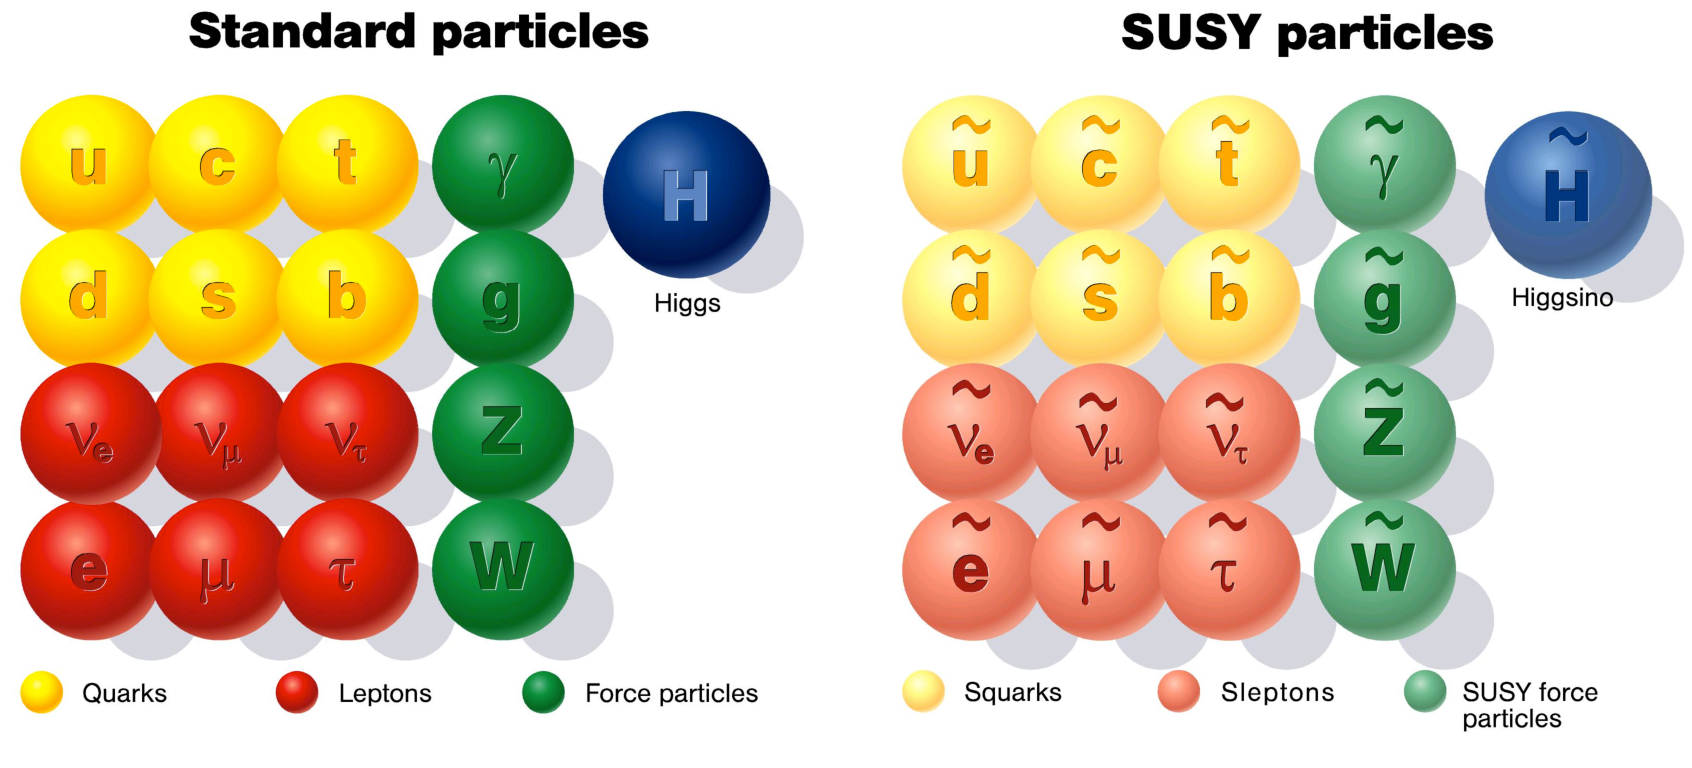
\includegraphics[keepaspectratio=true, scale=0.5]{./SM_SUSY_particles.pdf}
 % SM_SUSY_particles.jpg: 3478x1596 pixel, 300dpi, 29.45x13.51 cm, bb=0 0 835 383
 \caption[Supersymmetry particles.]{Supersymmetry partners (right) of the Standard Model particles (left).}
 \label{fig:SM_SUSY_Particles}
\end{figure}
\vspace{-0.01\textheight}

In the minimal supersymmetric extension of the \SM (MSSM) there can only be one such supermultiplet, but it has 105 unknown parameters (mass, angle, and phase parameters). The MSSM Lagrangian includes all possible supersymmetric interaction terms that satisfy SU(3)~$\times$ SU(2)~$\times$ U(1) gauge invariance and $B-L$ conservation, where $B$ is the baryon number and $L$ is the lepton number. The electric charge is defined by $Q=T_{3}+\frac{1}{2}Y$ where $T_{3}$ is the third component of the weak isospin and $Y$ is the hypercharge. The gauge supermultiplets consist of the gluons and their gluino fermionic superpartners and the gauge bosons and their gaugino fermionic superpartners. The extended Higgs sector of the MSSM is needed to guarantee cancellation of anomalies and to generate the desired quark masses. The corresponding field content of the MSSM and gauge quantum numbers are shown in Table~\ref{tab:SUSY_MSSM_Fields}.

\begin{table}
\caption{The particles (fields) in the MSSM and their quantum numbers. Only one generation of quarks and leptons are shown. For each lepton, quark, and Higgs supermultiplet, there is a corresponding antiparticle multiplet of charge-conjugated fermions and their associated scalar partners \cite{pap:PDG}.}
\label{tab:SUSY_MSSM_Fields}
\centering
\begin{tabular}{cccccc}
\hline
%\multicolumn{6}{c}{Field Content of the MSSM}\\
%\hline
\BUbf{Super-} & \BUbf{Boson} & \BUbf{Fermionic} & & & \\
\BUbf{Multiplets} & \BUbf{Fields} & \BUbf{Partners} & \BUbf{SU(3)} & \BUbf{SU(2)} & \BUbf{U(1)}\\
\hline
gluon/gluino & $g$ & $\widetilde{g}$ & 8 & 1 & 0\\[1ex]
gauge boson/ & $W^{\pm}$, $W^{0}$ & $\widetilde{W}^{\pm}$, $\widetilde{W}^{0}$ & 1 & 3 & 0\\
gaugino & $B$ & $\widetilde{B}$ & 1 & 1 & 0\\[1ex]
slepton/ & $(\widetilde{\nu},\widetilde{e}^{-})_{L}$ & $(\nu,e^{-})_{L}$ & 1 & 2 & --1\\
lepton & $\widetilde{e}^{-}_{R}$ & $e^{-}_{R}$ & 1 & 1 & --2\\[1ex]
squark/ & $(\widetilde{u}_{L},\widetilde{d}_{L})$ & $(u,d)_{L}$ & 3 & 2 & 1/3\\
quark & $\widetilde{u}_{R}$ & $u_{R}$ & 3 & 1 & 4/3\\
& $\widetilde{d}_{R}$ & $d_{R}$ & 3 & 1 & --2/3\\[1ex]
Higgs/ & $(H_{d}^{0}, H_{d}^{-})$ & $(\widetilde{H}_{d}^{0}, \widetilde{H}_{d}^{-})$ & 1 & 2 & --1\\
higgsino & $(H_{u}^{+}, H_{u}^{0})$ & $(\widetilde{H}_{u}^{+}, \widetilde{H}_{u}^{0})$ & 1 & 2 & 1\\[1ex]
\hline
\end{tabular}
\end{table}

\subsection{$R$-Parity}
Every SUSY particle is assigned a new quantum number called \newterm{R-parity}:
\begin{equation}
 R = (-1)^{3(B-L)+2S}
 \label{eqa:SUSY_Rparity}
\end{equation}
where $B$ ($L$) is its baryon (lepton) number and $S$ is the spin. The SM and the SUSY particles differ by this quantum number and all SM particles have $R=1$ while SUSY particles have $R=-1$. There are many extensions to SUSY based on conservation of or violation of $R$-parity. It is generally believed that $R$-parity is conserved as otherwise it can lead to an unacceptable fast proton decay. As a consequence, SUSY particles are produced in pairs, and a SUSY particle decays into SM particles accompanied by the lightest SUSY particle (LSP), which is proposed to be stable. Furthermore, cosmological constraints require that the LSP be neutral and colorless.

\subsection{Charginos and Neutralinos}
The mixing of the charged gauginos ($\widetilde{W}^{\pm}$) and the charged higgsinos ($H_{u}^{+}$ and $H_{d}^{-}$) is described by a complex $2\times2$ mass matrix (at tree-level) \cite{pap:SUSYCharginoMasses1, pap:SUSYCharginoMasses2}. This gives rise to non-negative chargino masses denoted by $\widetilde{\chi}^{\pm}_{1}$ and $\widetilde{\chi}^{\pm}_{2}$. These are linear combinations of the charged gaugino and higgsino states.

The mixing of the neutral gauginos ($\widetilde{B}$ and $\widetilde{W}^{0}$) and neutral higgsinos $\widetilde{H}_{u}^{0}$ and $\widetilde{H}_{d}^{0}$ is described by a complex symmetric $4\times4$ mass matrix (at tree level) \cite{pap:SUSYCharginoMasses1, pap:SUSYGauginoMasses1, pap:SUSYGauginoMasses2}. This gives rise to four physical neutralino states denoted by $\widetilde\chi_{i}^{0}$ ($i=1,..., 4$), where the states are ordered by increasing mass, $M_{\widetilde\chi_{1}^{0}} \leq M_{\widetilde\chi_{2}^{0}} \leq M_{\widetilde\chi_{3}^{0}} \leq M_{\widetilde\chi_{4}^{0}}$. The $\widetilde\chi_{i}^{0}$ are the linear combinations of the neutral gaugino and higgsino states.

\subsection{Breaking of SUSY}
There are many theory models that attempt to explain how the supersymmetry is broken so the expected masses and the interactions of the superpartners are acceptable. One of the leading candidates is the \newterm{Gauge Mediated Supersymmetry Breaking} (GMSB) method \cite{ pap:SUSY_SMartin, pap:SUSY_MDine1993}. In GMSB, SUSY is broken at very high energies, in a \newterm{hidden sector} that introduces SUSY-breaking interactions to the \newterm{visible} gauginos and scalars. Then, all SUSY counterparts are either heavier than their SM counterparts or are too weakly interacting.
In GMSB, the LSP is fixed to be the gravitino ($\widetilde{G}$). The $\widetilde{G}$ mass is typically in the eV range. The $\widetilde{G}$ is also considered as a potential dark matter candidate in the recent literature \cite{pap:DarkMatterCandidates}.

So far there has been no experimental evidence of superpartners. This could possibly be due to the inaccessibility of high masses with current particle accelerators. The Large Hadron Collider (LHC) at CERN has the potential of such discoveries as it reaches the design center of mass energy of 14~TeV over the next few years.

%%%%%%%%%%%%%%%%%%%%%%%%%%%%%%%%%%%%%%%%%%%%%%%%
% IDEA OF SIGNATURE BASED SEARCH
%%%%%%%%%%%%%%%%%%%%%%%%%%%%%%%%%%%%%%%%%%%%%%%%
\section{The Signature-Based Search}
Given the large number of theoretical models proposed with many free parameters, it is virtually impossible to test all of them explicitly. A \textit{signature-based} search is one way to search for new physics beyond the present theoretical understanding, which is currently described by the Standard Model. A signature is defined by the final-state particles --- those particles that we can measure in the detector. In a signature-based search, a certain decay process and decay products are studied by measuring the final-state particles. Starting with a certain level of understanding of the kinematics of the process, one examines kinematic distributions of the final-state particles for an anomalous behavior of observed data.

The selection of a signature has strong theoretical motivations. Incompleteness of the SM provides a tremendous motivation for a search like this. The selection of a signature is based on several factors. One deciding factor is the amount of data available with the required final-state particles. This will directly affect the precision of the final measurements and also the sensitivity. The detector's ability to identify and reconstruct particular particles will contribute. Another motivation for studying a particular signature might be inconclusive results of a previous study. For example, the recent inclusive photon + jet + $X$ (anything) cross section measurement has shown differences between data and theory \cite{pap:PhoJetCrosssection_D0}. Authors were unable to explain the dependence of the cross section on $p_{T}^{\gamma}$ over the whole measurement range.

There are many advantages to doing a signature-based search. Instead of optimizing the data analysis for a particular theoretical model and searching only a narrow region of phase space, one instead searches the entire phase space accessible via the data. By doing so, a global sensitivity to any anomaly, not just an anomaly associated with a particular theoretical model, can be achieved. Because the final measurement presents the behavior of the data as it is, the measurement never becomes obsolete and future models can even be tested using the data (provided there is complete information such as the efficiency and acceptance for measured objects). An added bonus of a signature-based search is that it can easily spawn new searches. A search can be easily expanded by requiring additional final-state objects. For example, a search for photon + jets can be extended to photon + electron + jet or photon + \particle{b}-quark jet.

There are some downsides to a signature-based search. Not optimizing for any particular model could mean less sensitivity to observing evidence for it. There is no measure of efficiency or the acceptance for objects associated with a decay mode. Hence, the final results may be less precise and less valuable to theorists.

\section{Photon + Jets Signature}
This thesis studies the physics of \ppbar collisions that produce a photon and jets as final-state particles. Section \ref{sec:gjetProdInSM} describes the production of a photon in the SM, which can lead to a photon + jets signature in the detector. During the initial parton interaction, a photon is radiated by the incoming or outgoing quark (antiquark). A photon produced directly from the incoming or outgoing quark (antiquark) is known as a \newterm{prompt photon}. The outgoing partons (quarks or gluons) will be observed as jets in the detector. Furthermore, it is possible for the incoming or outgoing partons to radiate extra gluons or photons, and those will be measured as additional jets and photons in the detector. However, such emissions are suppressed by the coupling strengths.

In the leading-order $2\to2$ SM process, the photon and jet are produced back-to-back in the center of mass frame of the incoming partons, as seen in Fig. \ref{fig:gjet_topology}. Because the incoming partons only have momentum along the $z$ axis, the momenta of the photon and jet must be balanced in the transverse plane.\footnote{The transverse plane is chosen for convenience of measurements. This eliminates the difficulty of measuring the longitudinal momentum of the incoming partons.} The presence of extra jets or photons will change this back-to-back topology. Also, it should be noted that SM $\gamma$ + jet processes show no undetectable particles that can produce an energy imbalance in the transverse plane.

\begin{figure}[htbm]
 \centering
\subfigure[]{\label{fig:gjet_toplogy_cm}
 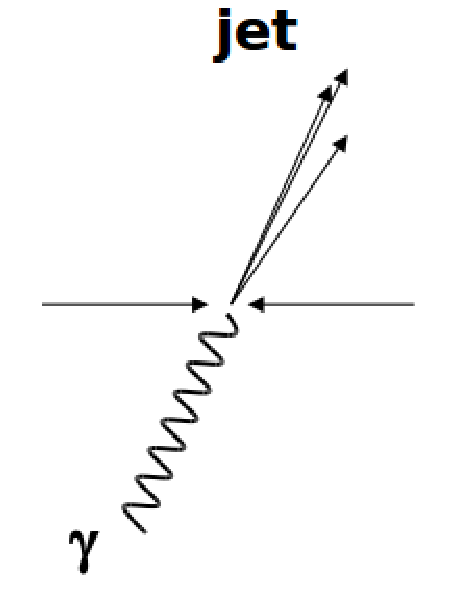
\includegraphics[scale=.6,keepaspectratio=true]{images/backtoback_gjet_cm_demo.pdf}
}
\subfigure[]{\label{fig:gjet_toplogy_lab}
 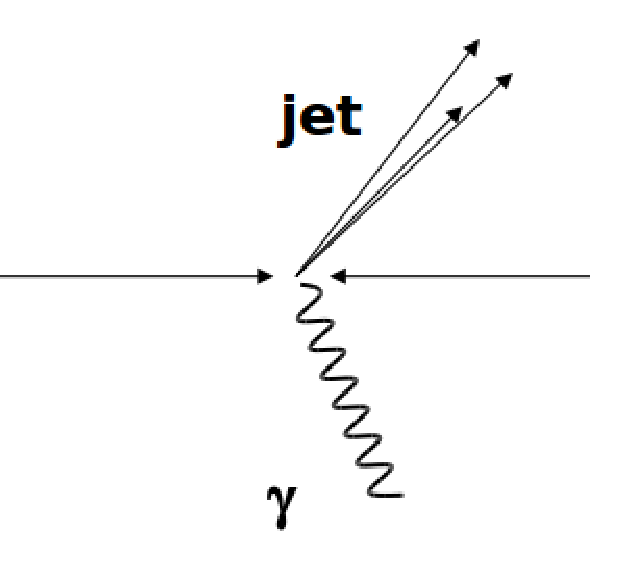
\includegraphics[scale=.6,keepaspectratio=true]{images/backtoback_gjet_lab_demo.pdf}
}
\caption{Topology of a $\gamma$ + jet event. (a) The $\gamma$ and jet are produced back-to-back in the center of mass frame of the incoming partons. (b) The $\gamma$ and jet are boosted (along the $z$ axis into lab frame).}
 \label{fig:gjet_topology}
\end{figure}
\vspace{-0.02\textheight}

The study of prompt photons has several advantages. Prompt photons emerge directly from the hard scattering process without undergoing fragmentation. Hence, by studying these photons, it is possible to extract parent parton information. Since the photon is a well understood elementary particle that interacts via the electromagnetic force, its energy can be measured with high accuracy to avoid a large systematic uncertainty associated with jet identification. Furthermore, photons are easier to identify using the detector's trigger system, and photon reconstruction is relatively simple.

By studying data events with a photon and jets, the presence of a new decay process or a new heavy particle may become evident by a sudden increase in the number of observed events in a narrow region of a distribution or distributions. A weakly interacting particle, like the hypothesized $\widetilde{G}$ in the decay of $\widetilde{\chi}^{0}_{1}\to\gamma \widetilde{G}$ in GMSB, is likely to produce an excess of data events with a large energy imbalance in the transverse plane.

\subsection{Photon + Jets Production in the SM}\label{sec:gjetProdInSM}

\begin{figure}[p]
\begin{center}
\subfigure[Annihilation]{
\label{fig:SM_pj_annihilation}
\begin{tabular}{cc}
\raisebox{0\height}{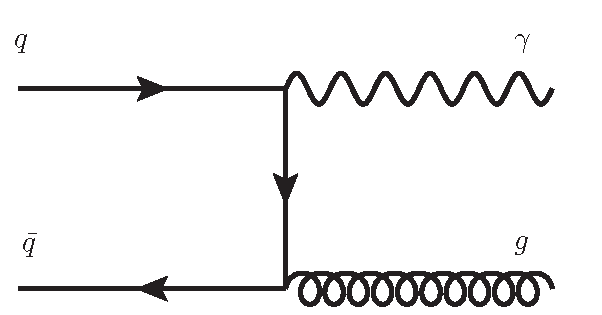
\includegraphics[scale=0.5]{images/Feyn_gjet_annihilation.pdf}} &
\raisebox{0\height}{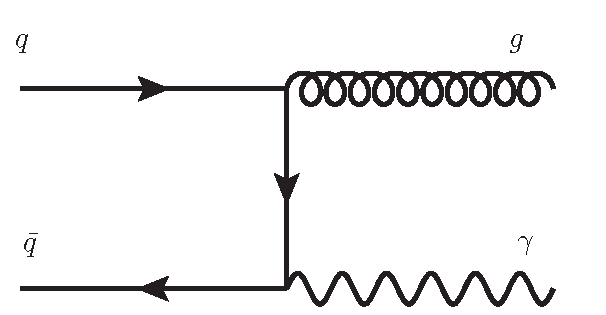
\includegraphics[scale=0.5]{images/gjets_qq2gpho_annihilation3.pdf}}\\
\multicolumn{2}{c}{\raisebox{0\height}{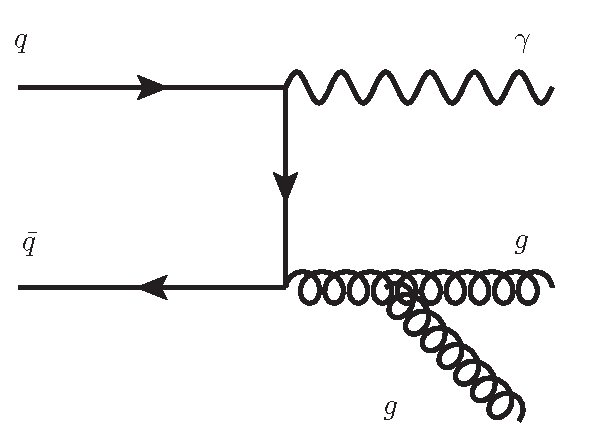
\includegraphics[scale=0.5]{images/Feyn_gjets_annihilation.pdf}}}
\end{tabular}
}
\subfigure[Compton Scattering]{
\label{fig:SM_pj_compton}
\begin{tabular}{cc}
\raisebox{0.1\height}{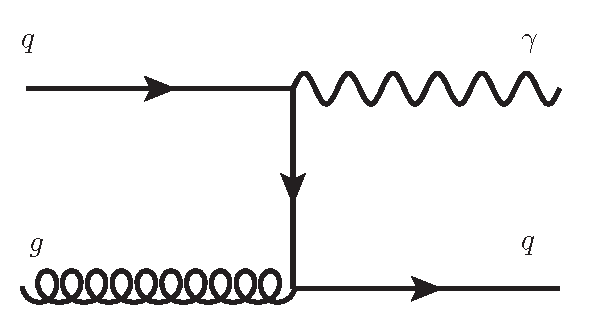
\includegraphics[scale=0.5]{images/Feyn_gjet_compton.pdf}} &
\raisebox{0.0\height}{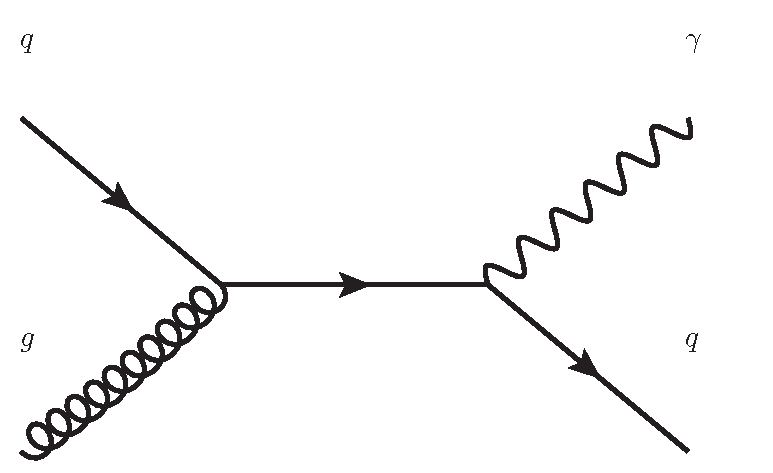
\includegraphics[scale=0.4]{images/gjets_qg2phoq_compton2.pdf}}\\
\raisebox{0.0\height}{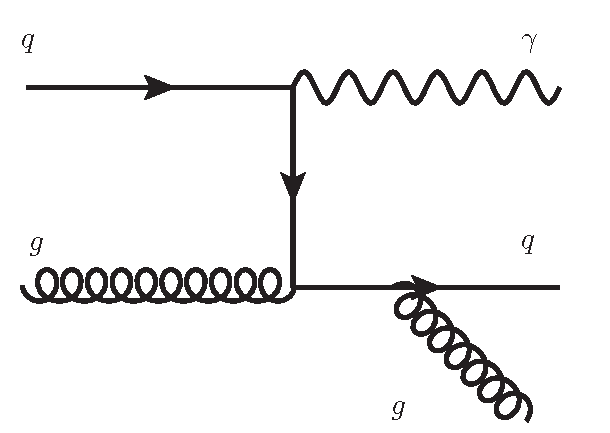
\includegraphics[scale=0.5]{images/Feyn_gjets_compton.pdf}}&
\raisebox{0.0\height}{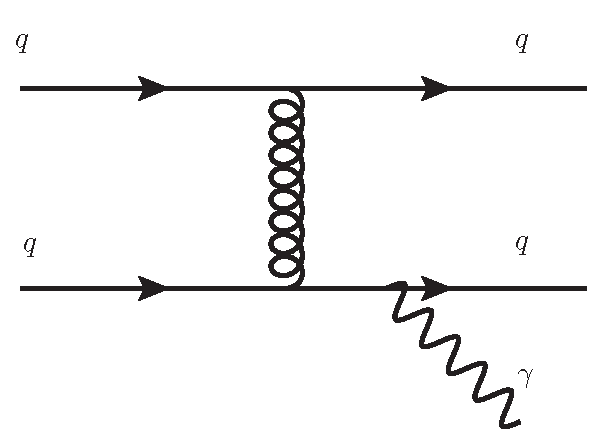
\includegraphics[scale=0.5]{images/gjets_qq2qq_compton.pdf}}
\end{tabular}
}
\subfigure[Bremsstrahlung Radiation]{
\label{fig:SM_pj_brem}
\begin{tabular}{cc}
\raisebox{0.3\height}{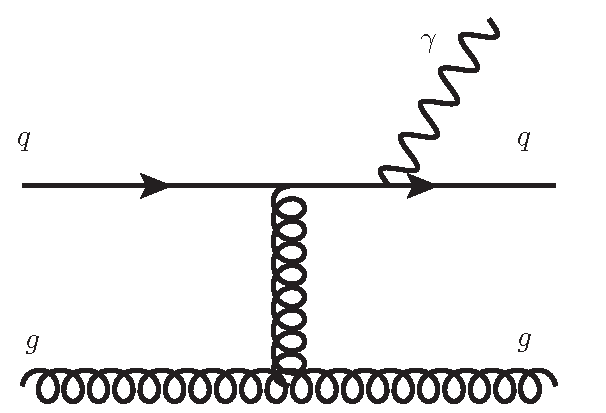
\includegraphics[scale=0.5]{images/Feyn_gjet_brem.pdf}} &
\raisebox{0.0\height}{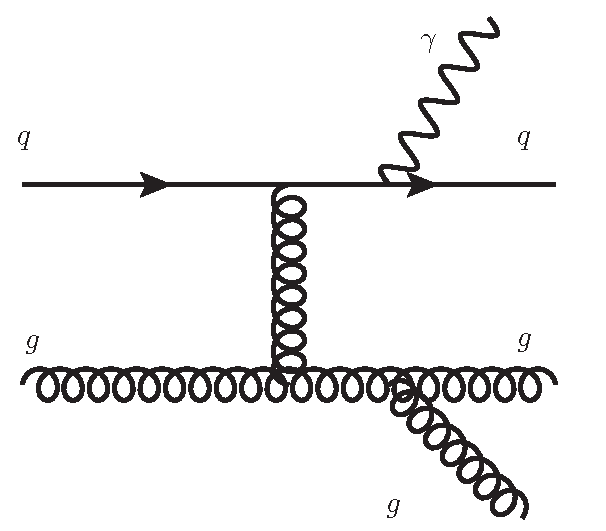
\includegraphics[scale=0.5,keepaspectratio=true]{images/Feyn_gjets_brem.pdf}}
\end{tabular}
}
\end{center}
\caption{Leading-order and next-to-leading-order Feynman diagrams for Standard Model prompt photon production. Next-to-leading-order production will have extra gluon radiation and/or gluon exchanges.}
\label{fig:SM_pj_Feynmans}
\end{figure}

The SM production of photons ($\gamma$) is a radiative process in which a photon is emitted either from an initial-state parton or from a final-state parton. This can happen only through a quark, which is electrically charged and can couple to a photon via the electromagnetic interaction (QED). The partons (quarks and/or gluons) will proceed to interact via the strong force. This prompt photon production can be divided into two components, a direct component (Fig.~\ref{fig:SM_pj_annihilation} and Fig.~\ref{fig:SM_pj_compton}) and bremsstrahlung (Fig.~\ref{fig:SM_pj_brem}). To lowest order, at large photon momentum, the inclusive cross section is dominated by the following two subprocesses:
\begin{eqnarray}
\mathrm{Compton:} && q(\bar{q}) + g \to \gamma + q(\bar{q})\\
\mathrm{Annihilation:} && q + \bar{q} \to \gamma + g
\label{eqa:gjets_ComptAnnihilation}
\end{eqnarray}
To lowest order, the invariant cross section for the subprocess
\begin{equation}
 a+b\to c+\gamma
\end{equation}
can be written as
\begin{equation}
 E_{\gamma}\frac{d\hat{\sigma}}{d^{3}p_{\gamma}} = \frac{\hat{s}}{\pi}\frac{d\sigma}{d\hat{t}}\delta(\hat{s}+\hat{t}+\hat{u})
\end{equation}
where $\hat{s}$, $\hat{t}$, and $\hat{u}$ are the Mandelstam variables \cite{pap:JFOwens_RevModPhy59465_1987} for the subprocess. The elementary cross sections for the leading-order processes (${\cal O}(\alpha_{s})$) are
\begin{eqnarray}
 \frac{d\sigma}{d\hat{t}} (q + g \to \gamma + q) &=& -\frac{\pi\alpha\alpha_{s}}{3{\hat s}^{2}} e^{2}_{q} \frac{{\hat u}^{2}+{\hat s}^2}{{\hat u}{\hat s}}\\
 \frac{d\sigma}{d\hat{t}}(q + \bar{q} \to \gamma + g) &=& -\frac{8\pi\alpha\alpha_{s}}{9{\hat s}^{2}} e^{2}_{q} \frac{{\hat u}^{2}+{\hat t}^2}{{\hat u}{\hat t}}
\end{eqnarray}
where $e_{q}$ is the charge of the interacting quark. Although the two components are topologically distinct, interference effects make them inseparable. Still, one can gain insight into these processes by measuring the separation between the objects and the softness of their energies.

Isolated photons from photon + jets production come largely unaltered from the hard scattering process. Hence, they can be used to directly probe the hard scattering dynamics. At low transverse momentum of the photon, the Compton scattering process $qg\to q\gamma$ dominates. This process probes the gluon density of the colliding hadrons at low momenta where gluons carry the bulk of the momentum. At higher transverse momenta, quark and antiquark annihilation $q{\bar q}\to g\gamma$ becomes the dominant process.

Final-state quarks and gluons will hadronize to form stable particles, and will be observed as a collimated spray of particles called a jet. At the detector level, these events would be reconstructed as a photon plus one or more jets. The initial-state and final-state partons can radiate additional gluons to produce more jets.

The emission of a $\gamma$ is due to a point-like QED coupling that provides a unique opportunity to study the partons more closely, specifically the gluon content of the protons and antiprotons.

It is important to note that there is no intrinsic missing energy present in these processes. Any measured missing energy would be most likely due to mismeasurements. But a significant number of events with large missing energy could also indicate new physics.

\begin{figure}[htbm]
 \centering
 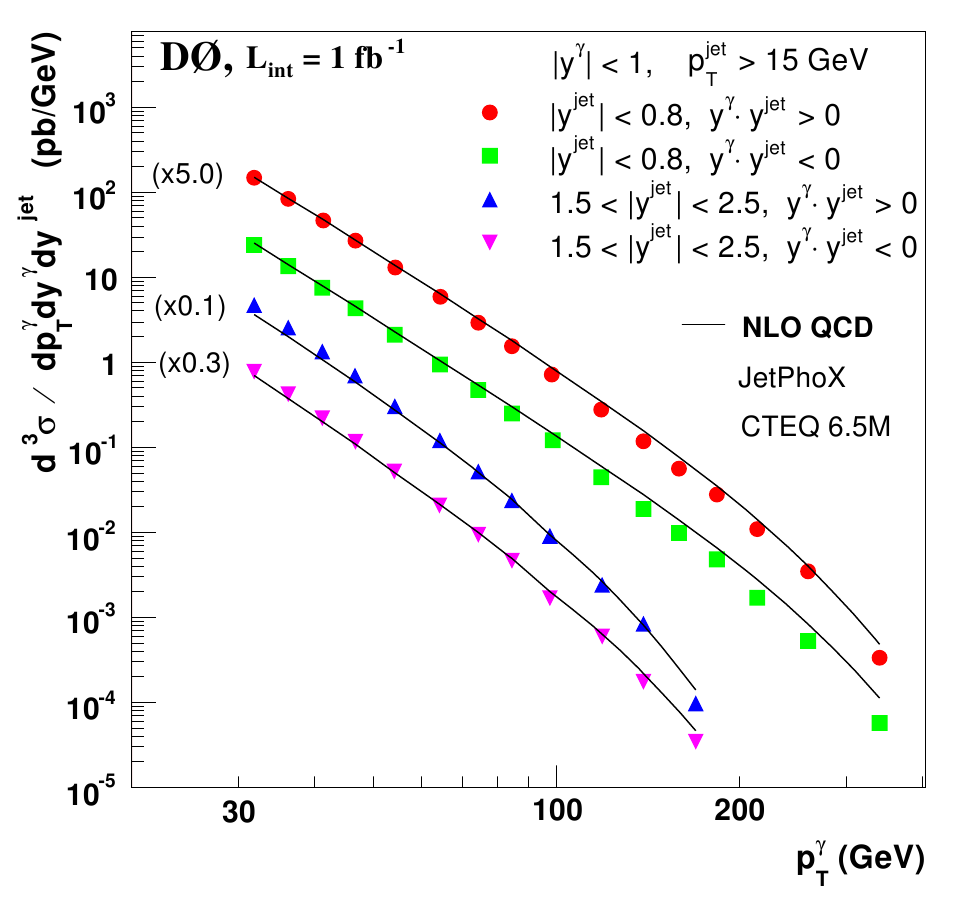
\includegraphics[scale=0.45,keepaspectratio=true]{./PhoJets_Crosssection.png}
 % PhoJets_Crosssection.png: 646x612 pixel, 96dpi, 17.09x16.19 cm, bb=0 0 484 459
 \caption{Differential cross section of $\ppbar\to\gamma+\mathrm{jet}+X$ measured as a function of the transverse energy of the photon $p_{T}^{\gamma}$. $X$ represents any other physics object(s) not identified in the event. The photon is required to have \ptg{30.0} and \etalessthan{1.0}, and the jet is required to have \ptg{15.0} and \etalessthan{2.5}. Cross sections are measured in four regions of rapidity $y$. For presentation purposes, some distributions are scaled by the factors shown along the side of each curve. The black lines correspond to the theoretical predictions
 \cite{pap:PhoJetCrosssection_D0}.}
 \label{fig:PhoJetCrosssection}
\end{figure}
\vspace{-0.02\textheight}

Figure~\ref{fig:PhoJetCrosssection} describes a recent measurement of the photon + jets cross section as a function of the transverse energy of the photon. It is worth comparing the scale of the photon + jets cross section to the cross section for jet production shown in Fig.~\ref{fig:ProductionCrosssections}. Figure~\ref{fig:ProductionCrosssections} shows the cross sections of some of the physics processes at different center of mass energies. These probabilities depend on the luminosity as demarcated on the right hand axis. This example shows the overwhelmingly large number of physics processes and the difficulty of isolating rare processes.

\begin{figure}[htmb]
 \centering
 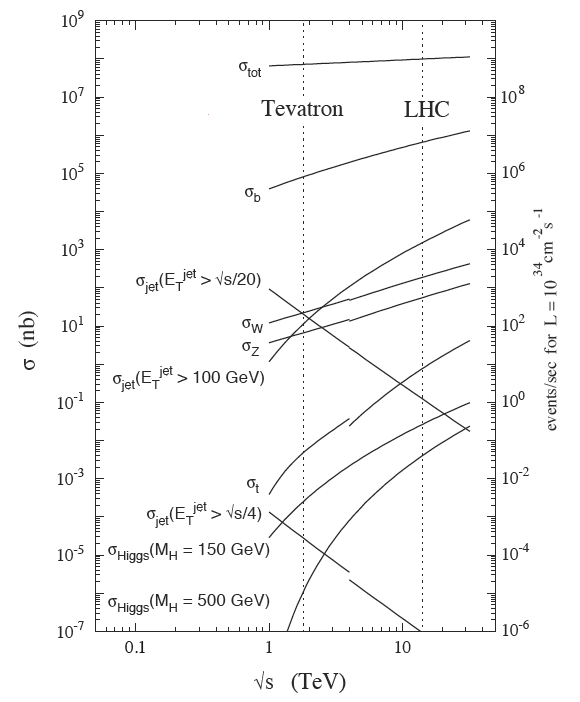
\includegraphics[scale=0.55,keepaspectratio=true]{./ParticleCrossSections.png}
 % ParticleCrossSections.pdf: 408x518 pixel, 72dpi, 14.39x18.27 cm, bb=0 0 408 518
 \caption{Cross sections for some physics processes at the Large Hadron Collider (LHC) at CERN \cite{www:LHCPublic} and the Tevatron at Fermilab \cite{www:FNALpublic}. The dotted lines show the energies of the two hadron colliders: 14~TeV at the LHC at 14~TeV and 1.96~TeV at the Tevatron \cite{www:ParticleProductionCrosssections}. Discontinuities seen for certain processes are due to the difference in colliding beams. At the LHC proton-proton beams are collided, whereas at the Tevatron proton-antiproton beams are collided. Processes dominated by gluon interactions are not changed, but the processes dominated by quarks do change, as seen by the discontinuities.}
 \label{fig:ProductionCrosssections}
\end{figure}


\subsection{Photon + Jets Production in \GMSBtext}
The Feynman diagrams shown in Fig.~\ref{fig:GMSBSUSY} show GMSB processes in which a photon and a jet(s) are produced in the final state. The SUSY particles decay into SM particles via a cascade decay. This decay will be observed as follows. A photon will be produced by $\widetilde{\chi}^{0}_{1}\to \gamma\widetilde{G}$ and the $\widetilde{G}$ will escape detection, producing a large energy imbalance. One or more of the other decay products ($\tau$) will be identified as jet(s). Using these decay products it is possible to measure the mass of the SUSY particles.

\begin{figure}[hbt!]
 \centering

\subfigure[]{
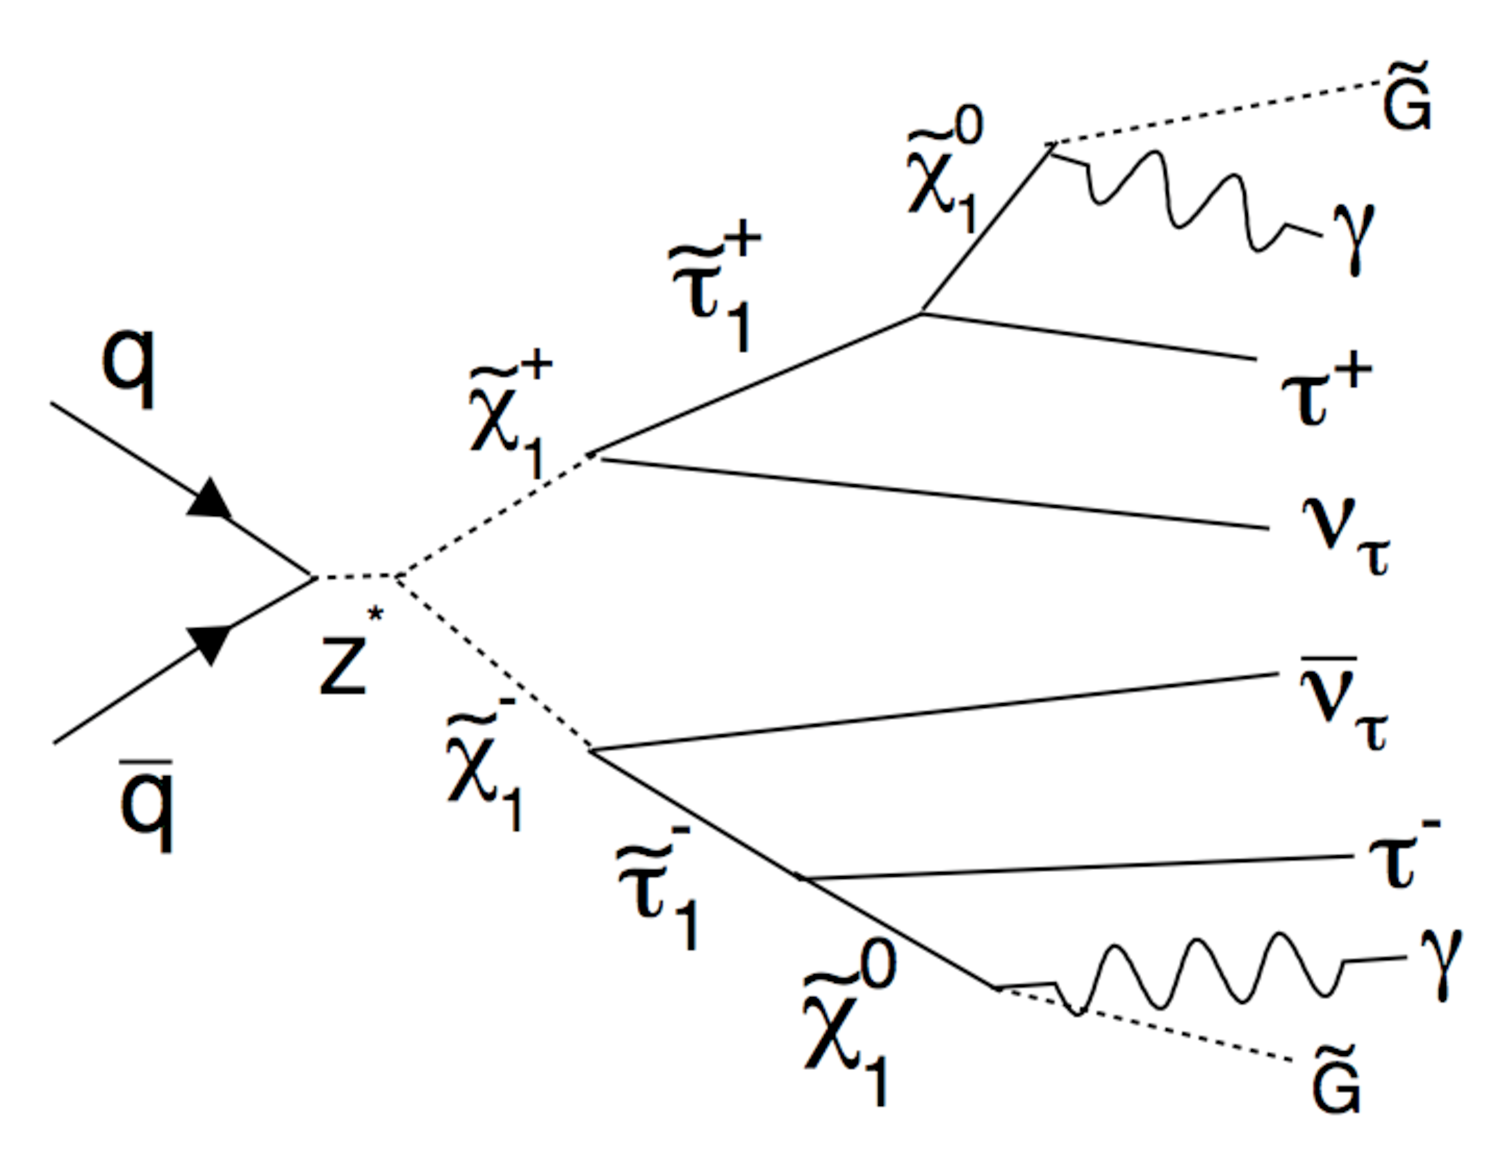
\includegraphics[scale=0.25]{images/SUSY_1.pdf}
\label{fig:SUSY_1}
}
\subfigure[]{
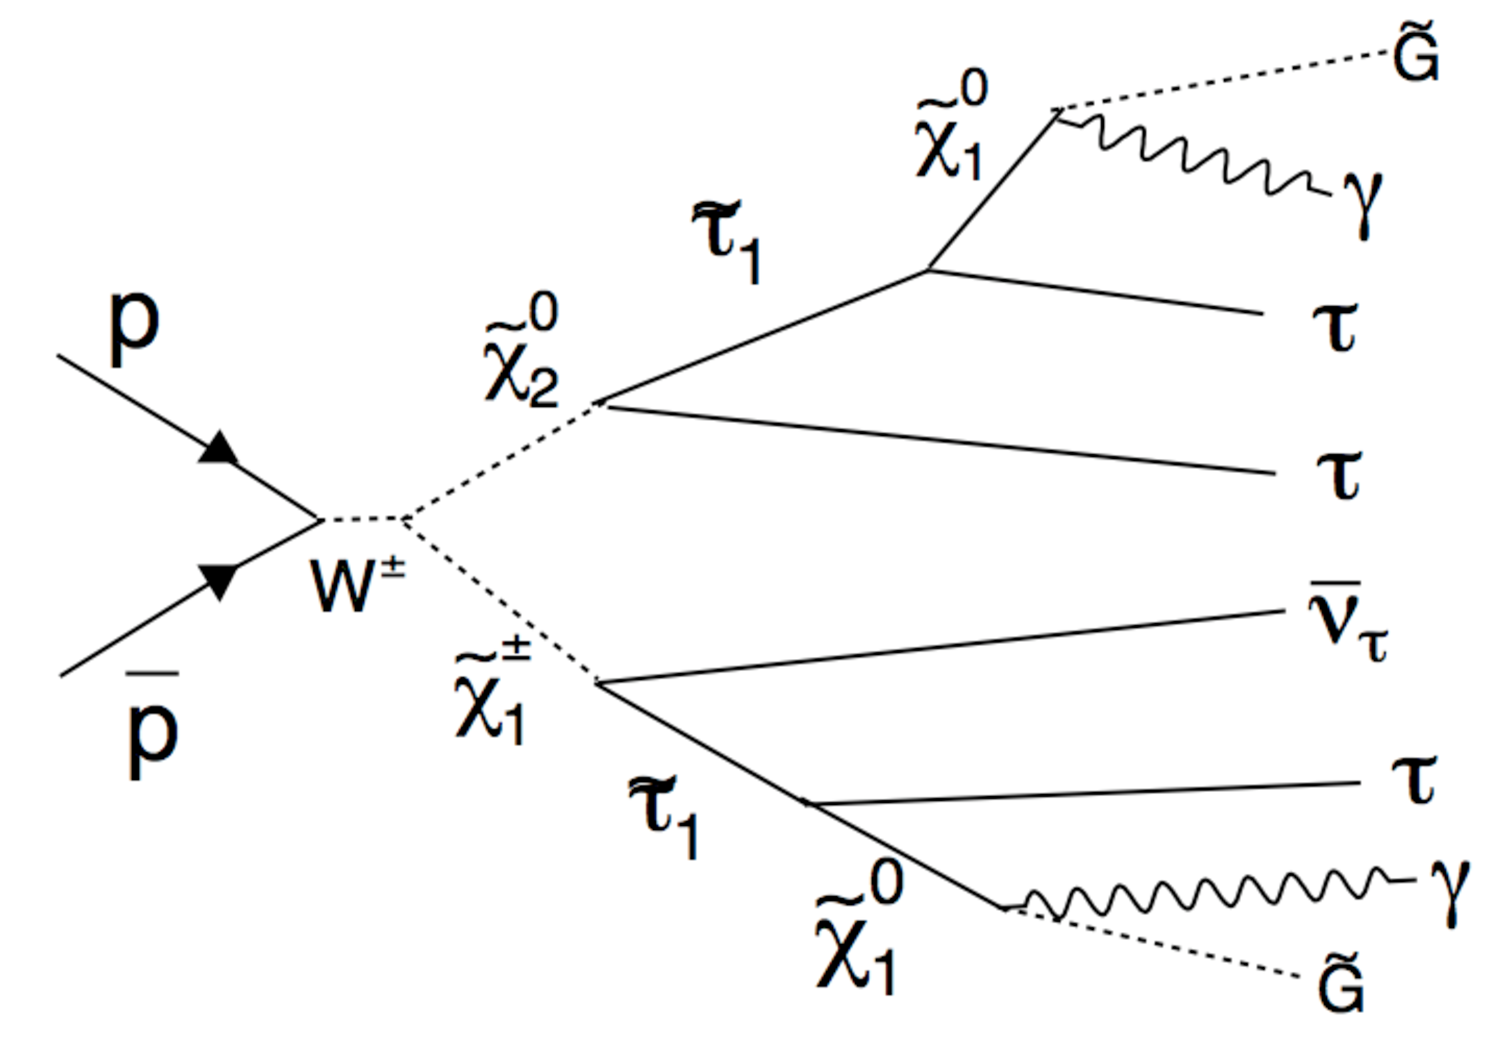
\includegraphics[scale=0.26]{images/SUSY_2.pdf}
\label{fig:SUSY_2}
}

 \caption{Predicted tree-level production mechanisms of GMSB theory.}
 \label{fig:GMSBSUSY}
\end{figure}
